\section{Single Shooting}
The optimization problem can be formulated as an nlp with the system dynamics as constraints. To avoid persistent strict policies, the cost function decreases quadratically with $u_k$. This can be viewed as a penalty modelling the negative impacts of lockdown.

\begin{mini*}|s|
{w}{\sum_{k=1}^NI_k^2 -W_u u_{k-1}^2 \triangleq \Phi(w)}
{}{}
\addConstraint{x_f = f(x_0, [u_0, \dots, u_{N-1}])}
\addConstraint{u_{max} \geq u_k \geq u_{min}}{}
\end{mini*}
Where $f(.)$ is the trajectory from initial to end state. The intermediate states of the system is not visible to the solver. $f(.)$ can be implemented as an iterative RK4-scheme:

\begin{algorithm}[H]
\SetAlgoLined
\KwData{$x_k = x_0, u = [u_0, \dots, u_{N-1}], h, N$}
define f as a RK4-integrator repeated M times\\
 \For{$i$ = 0 : $N-1$}{
    $x_k, Q_k = RK4(@SIR,@Cost, x_k, u_k, h)$\\
    $J += Q_k$\\
    add $u_{min} - u_k, u_k - u_{max}$ to bounds\\
    set $u_{k,0}$
 }
 \KwRet{$x_k, J, U_0$, bounds}
 \caption{Single-shooting problem construction and integration}
 \label{alg:SingleShooting_Integraion}
\end{algorithm}

The resulting variables, values and boundaries can be directly inserted into the CasADI-interface if derived symbolically, or directly intefaced with a solver when derived numerically.
\iffalse
\subsection{Optimal Control using IPOPT interfaced by CasADI}
The problem is formulated using CasADI in Python, where a single step of algorithm \ref{alg:SingleShooting_Integraion} is formulated with MX-symbolics and transformed to a CasADI-function. $u = [u_0, \dots, u_{N-1}]$ is initialized as a MX-variable and elementwise inserted into the function for each for-loop step in algorithm \ref{alg:SingleShooting_Integraion}. Boundaries are added to $u$, resulting in lists which can be inserted into the CasADI's solver framework.

Optimal control is solved using default parameters and initial conditions from \ref{ch:Problem_Parameters}.

\fi



\subsection{Primal-Dual Interior Point Formulation}
\subsubsection{KKT Conditions}
The inequalities can be replaced using the log-barrier method:

\begin{mini*}|s|
{w_\tau}{\Phi(w_\tau) - \tau \sum_{k=0}^{N-1}(\log(u_k-u_{min}) + \log(u_{max}-u_k))}
{}{}
\addConstraint{x_f = f(x_0, [u_0, \dots, u_{N-1}])}
\end{mini*}
\begin{align}
    h(w_\tau) &= \begin{bmatrix} u_0-u_{min} \\ u_{max}-u_0 \\ \vdots \\
u_{max}-u_{N-1}
    \end{bmatrix}& 
 \nu&= -\tau \begin{bmatrix}
h_0^{-1}\\ \vdots \\ h_{2(N-1)}^{-1} \end{bmatrix}
\end{align}
Which gives the Primal-Dual KKT-conditions:
\begin{align}
    \nabla \Phi(w) + \nabla h(w)\nu + \nabla f(x_0, [u_0, \dots, u_{N-1}])\lambda &= 0\nonumber \\
    g(w) = x_f-f(x_0, [u_0, \dots, u_{N-1}]) &= 0\\\nonumber
    \nu_ih_i(w) + \tau &= 0 \\\nonumber
    h(w) < 0, \nu &> 0
\end{align}
The complementarity slackness in the Primal-Dual method approximates the constraints for the original formulation, and will converge to $\mu$ for small $\tau$. The current formulation requires $h(w) < 0$, which can be relaxed with slack variable $s$. Furthermore, the problem can be expressed in terms of true KKT conditions by setting $\nu = \mu$, which upper bounds the optimum error $\mu^*-\nu^*$ linearly with $\tau$. This results in equation \ref{eq:KKT_approx_IPOPT}, where the equalities can be used for Newton-Rhapson steps.

\begin{align}
        \nabla \Phi(w) + \nabla h(w)\nu + &\nabla f(x_0, [u_0, \dots, u_{N-1}])\lambda = 0 \nonumber \\ 
        g(w) &= 0\nonumber \label{eq:KKT_approx_IPOPT}\\
    h_i(w) + s_i &= 0\\\nonumber
    \mu_is_i-\tau &= 0\\\nonumber
    s > 0, \mu &> 0
\end{align}

\subsubsection{Line Search}
In the case where the end-state of the trajectory is unconstrained, $g(w)$ can be omitted. The solution for each KKT problem can be found by using the Newton-Rhapson method on the KKT conditions. 
\begin{align}
    r(w, \mu, \tau) &= \begin{bmatrix}
    \nabla \mathcal{L}(w, \mu)\\
    h(w) + s\\
    \mu_is_i - \tau
    \end{bmatrix} = 0\\
    \begin{bmatrix}
    d^w\\d^\lambda\\d^\mu
    \end{bmatrix} &= \nabla r(w, \mu, \tau)^{-1} r(w, \mu, \tau)
\end{align}

It is not possible to guarantee invertibility of $r$ for the SIR-model due to nonlinear dynamics. [\cite{IPOPT_output_ref}] suggests ensuring invertibility by adding a diagonal term $\delta_w$ to the hessian of the lagrangian $\nabla_{ww}\mathcal{L}(w, \mu)$ in $\nabla r(w,\mu, \tau)$.

The steps can be constrained to decrease $r(w, \mu, \tau)$ at every iteration with the fraction-to-the-boundary rule:
\begin{align}
    \alpha_k^{max} &= \max \{\alpha \in (0,1]: w_k + \alpha d_k^w \geq (1-\tau_j)x_k\}\\
     \alpha_k^{\mu} &= \max \{\alpha \in (0,1]: \mu_k + \alpha d_k^\mu \geq (1-\tau_j)\mu_k\}\\
\end{align}
Where $w$ and $\lambda$ are updated according to $\alpha_k^{max}$, and $\mu$ according to $\alpha^\mu$.



\subsection{Sequential Quadratic Programming Formulation}
The problem can be approximated using the hessian of the lagrangian combined with the gradient of the objective, constraint and inequalities:
\begin{align}
    \mathcal{L}(x, \lambda, \mu) = \sum_{k=1}^NI_k^2 -W_u u_{k-1}^2 - \lambda g(w) - \mu h(w)
\end{align}

\begin{mini}|s|
{d}{\frac{1}{2}d^T \nabla^2_{ww}\mathcal{L}\mathcal(w) d + \nabla \Phi(w)^T d}
{}{}
\addConstraint{\nabla g(w)^T d + g(w) = 0}
\addConstraint{\nabla h(w)^T d + h(w) \leq 0}{}
\end{mini}
\subsubsection{Active Set Strategy}
After determining the current active inequality constraints, the the sequential step and multipliers can be determined from the Karush-Kuhn-Tucker conditions of the problem (Considering the approximated active inequalities $\nabla h_A(w)^T d + h_A(w) \leq 0$ as equality constraints with multiplier $\mu$).
\begin{equation}
    \begin{bmatrix}
    \nabla_{ww}\mathcal{L}(w, \lambda, \mu) & \nabla g(w) & \nabla h_A(w)\\
    \nabla g(w)^T & 0 & 0\\
    \nabla h_A(w)^T & 0 & 0
    \end{bmatrix}
    \begin{bmatrix}
    d\\
    \lambda\\
    \mu_A
    \end{bmatrix}= 
    -\begin{bmatrix}
    \Phi(w)\\
    g(w)\\
    h_A(w)
    \end{bmatrix}
\end{equation}

In the SIR-problem formulation we have the following boundary inequalities:
\begin{align}
    h(w) &= \begin{bmatrix} u_0-u_{min} \\ u_{max}-u_0 \\ \vdots \\
u_{max}-u_{N-1}
    \end{bmatrix} & \nabla h(w) &= \begin{bmatrix} 1 \\ -1 \\ \vdots \\1\\
-1
    \end{bmatrix}
\end{align}
Determining the active set for boundaries is simpler than for other inequalities, since they come in pairs where only one can be active at each iteration.

In the case of independent inequality constraints, the active set has to be determined by testing different steps with different active inequalities until positive multipliers and a feasible step has been achieved.

\subsection{IPOPT with CasADI's Symbolical Framework}
A single-shooting optimization problem was formulated with CasADI using the symbolical framework, for all three control strategies. Algorithm \ref{alg:PDIPOPT_CasADI_SYM} summarizes the basic loop for converging without $\delta$ or step-corrections.


\begin{algorithm}[H]
\SetAlgoLined
\KwData{$w = w_0 \in \mathbb{R}^{N_u + N_\mu + N_s}, \tau = 1, \tau_{min} = 1\times 10^{-3}, \Delta w_{tol} = 1\times 10^{-4}$}
\While {$(\tau > \tau_{tol})$ and $(\Delta w > \Delta w_{tol})$}{

    \While {$w_k > w_{k, tol}$}{

        $w_k = w_k - \nabla r(w, \mu, \tau)^{-1} r(w, \mu, \tau)$


    \EndWhile}

    $\Delta w = w_k - w_{k, old}$

    $\tau = 0.9\tau$

\EndWhile}

 \KwRet{$w_k$}
 \caption{Primal-Dual Interior Point with CasADI symbolical framework}
 \label{alg:PDIPOPT_CasADI_SYM}
\end{algorithm}

\subsubsection{Social Distancing}

Reducing step lengths using the fraction-to-the-boundary rule resulted in a very slow convergence with very small steps in $\alpha_k^\mu, \alpha_k^{max}$. While using $\delta$ and small steps is keeping $\nabla r(w, \mu, \tau)$ invertible, it does not converge towards a local optimal solution.

\subsubsection{Vaccination}

Optimization with vaccination policy was solvable without $\delta$ and step-corrections.

\begin{figure}[H]
    \centering
    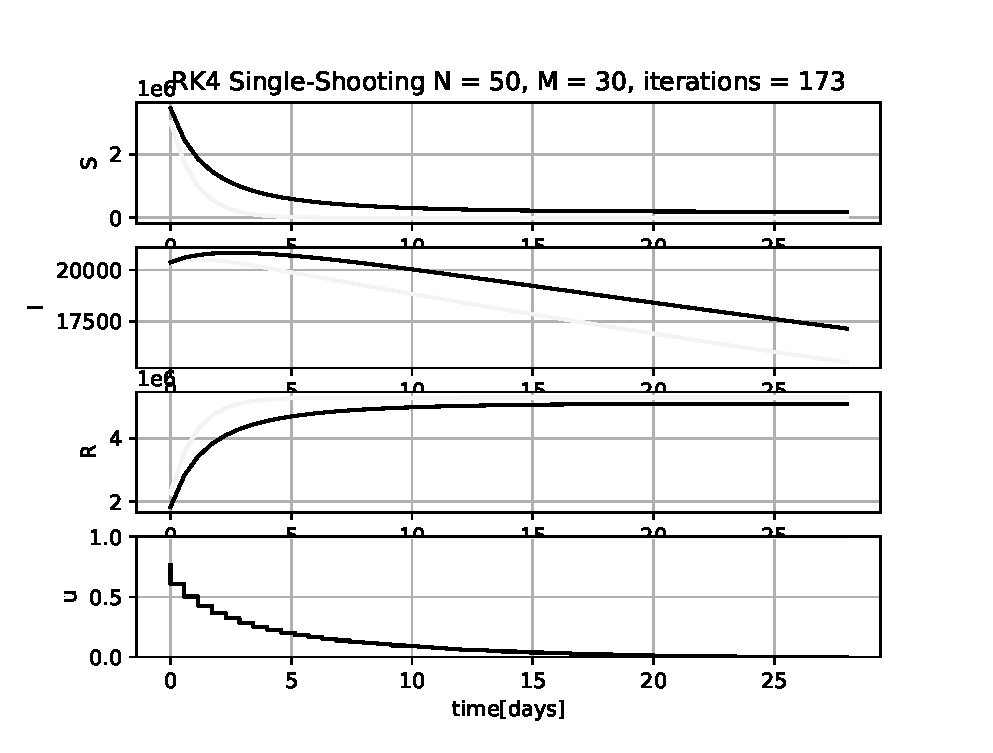
\includegraphics[width=.8\textwidth]{pythonProject/Figures/Symbolic_IPOPT_Traj_Vaccination.eps}
    \caption{Vaccination trajectories using Symbolical DP-IPOPT}
    \label{fig:Symbolical_DPIPOPT_traj_Vaccine}
\end{figure}
Figure \ref{fig:Delta_wk_convergence_Vaccine} shows the convergence of $\Delta w_k$.

\begin{figure}[H]
    \centering
    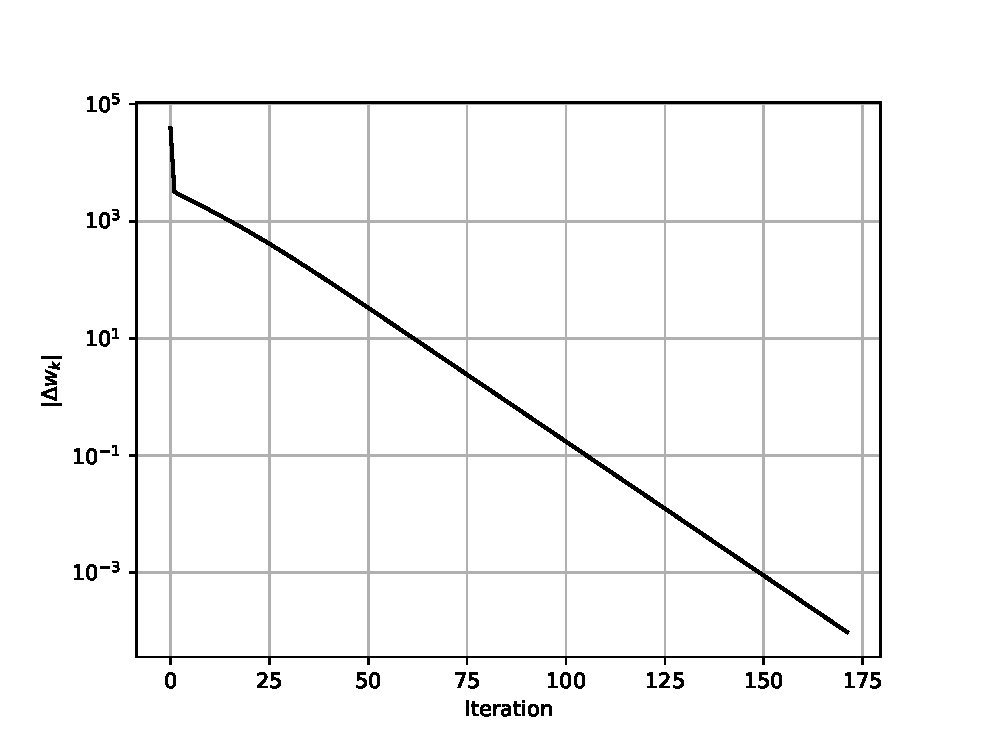
\includegraphics[width=.8\textwidth]{pythonProject/Figures/Symbolic_IPOPT_error_Vaccination.eps}
    \caption{$\Delta w_k$-convergence (Vaccine)}
    \label{fig:Delta_wk_convergence_Vaccine}
\end{figure}

\subsubsection{Isolation}

Optimization with isolation policy was solvable without $\delta$ and step-corrections.

\begin{figure}[H]
    \centering
    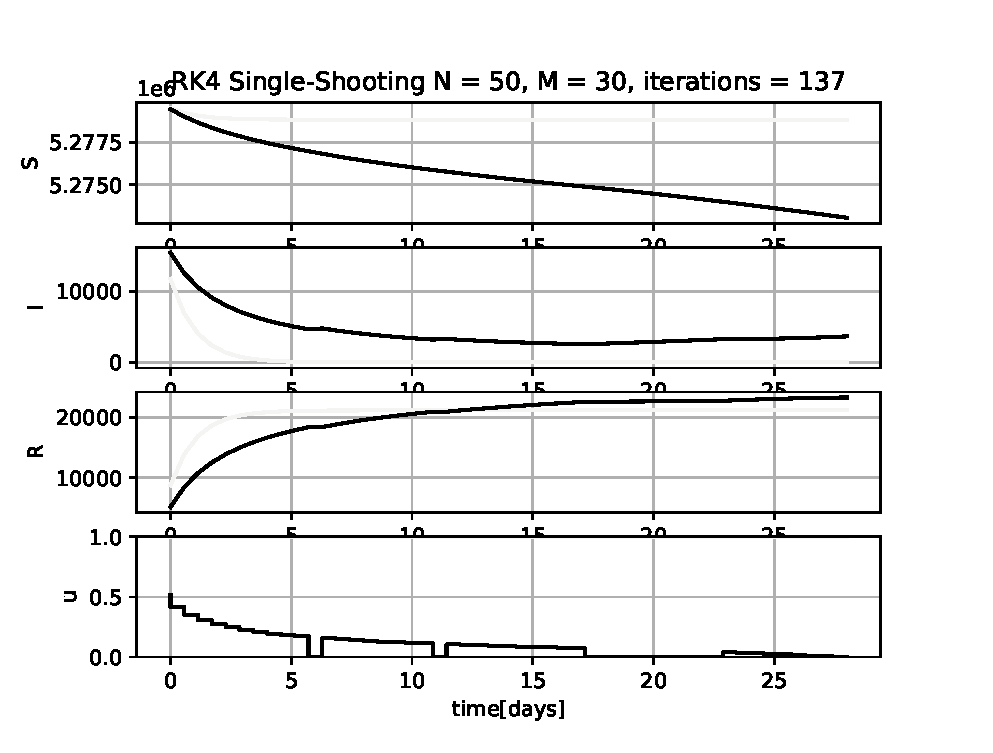
\includegraphics[width=.8\textwidth]{pythonProject/Figures/Symbolic_IPOPT_Traj_Isolation.eps}
    \caption{Isolation trajectories using Symbolical DP-IPOPT}
    \label{fig:Symbolical_DPIPOPT_traj_Vaccine_Isolation}
\end{figure}
Figure \ref{fig:Delta_wk_convergence_Isolation} shows the convergence of $\Delta w_k$.

\begin{figure}[H]
    \centering
    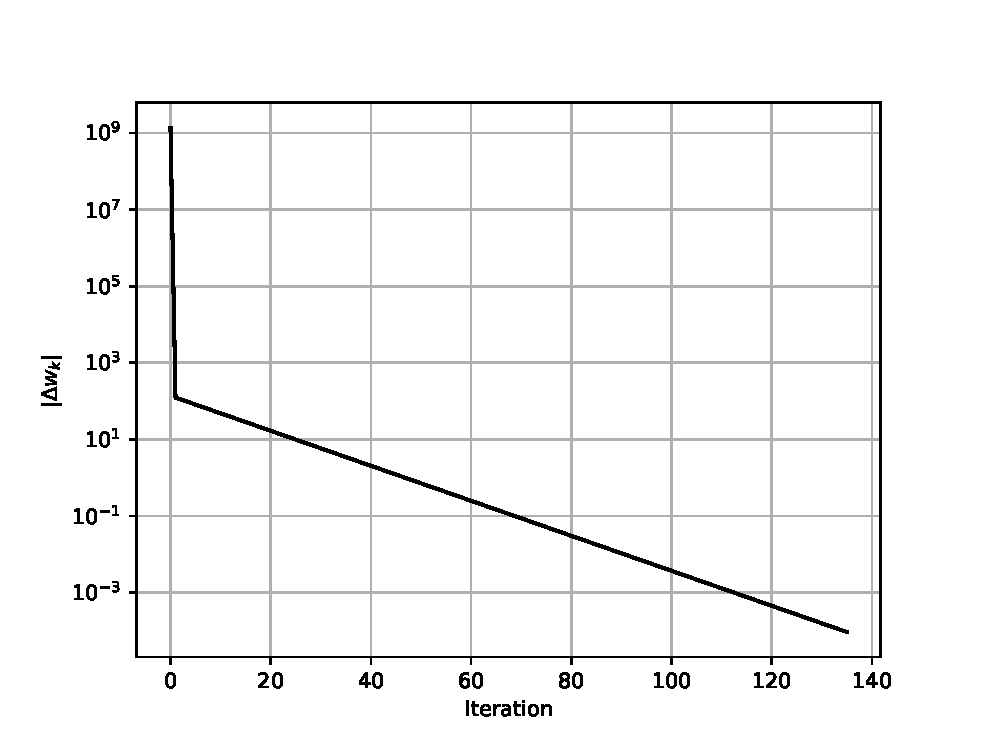
\includegraphics[width=.8\textwidth]{pythonProject/Figures/Symbolic_IPOPT_error_Isolation.eps}
    \caption{$\Delta w_k$-convergence (Isolation)}
    \label{fig:Delta_wk_convergence_Isolation}
\end{figure}


\subsection{Interfacing IPOPT in CasADI}
\subsubsection{Implementation}
Single-shooting is implemented in CasADI using $X_0 \in \mathbb{R}^3, U \in \mathbb{R}^{N}$ as MX-variables. The ODE is integrated $M$ times for each control interval, resulting in a total of $N\times M$ integration steps. Inequality constraints are passed as variable bounds, while equality constraints are passed as regular constraints to the solver.

\begin{algorithm}[H]
\SetAlgoLined
\KwData{$x_k = x_0, U = MX \in \mathbb{R}^{N}, J=0, h, N$}
Construct integrator $f(ODE, x, u, h)$ with CasADI-symbolics\\
 \For{$i$ = 0 : $N-1$}{
    $x_k, Q_k$ = $f([@SIR, @Cost\_ODE], x_k, U[i], h)$\\
    $J+= Q_k$\\
    add $u_{min} - u_k, u_k - u_{max}$ to bounds\\
    set $u_{k,0}$
 }
 solver = nlpsol('solver', 'ipopt', $\{$J, $U\}$)\\
 sol = solver($U_0$,bounds)
 \caption{Single-shooting with IPOPT}
 \label{alg:SingleShooting_Integration_IPOPT}
\end{algorithm}
\subsubsection{Social Distancing}
Simulating with parameters defined in section \ref{ch:Problem_Parameters} yields trajectories shown in figure \ref{fig:SH_Traj_IPOPT} and multiplier and objective values shown in figure \ref{fig:SH_con_obj_IPOPT}.

\begin{figure}[H]
    \centering
    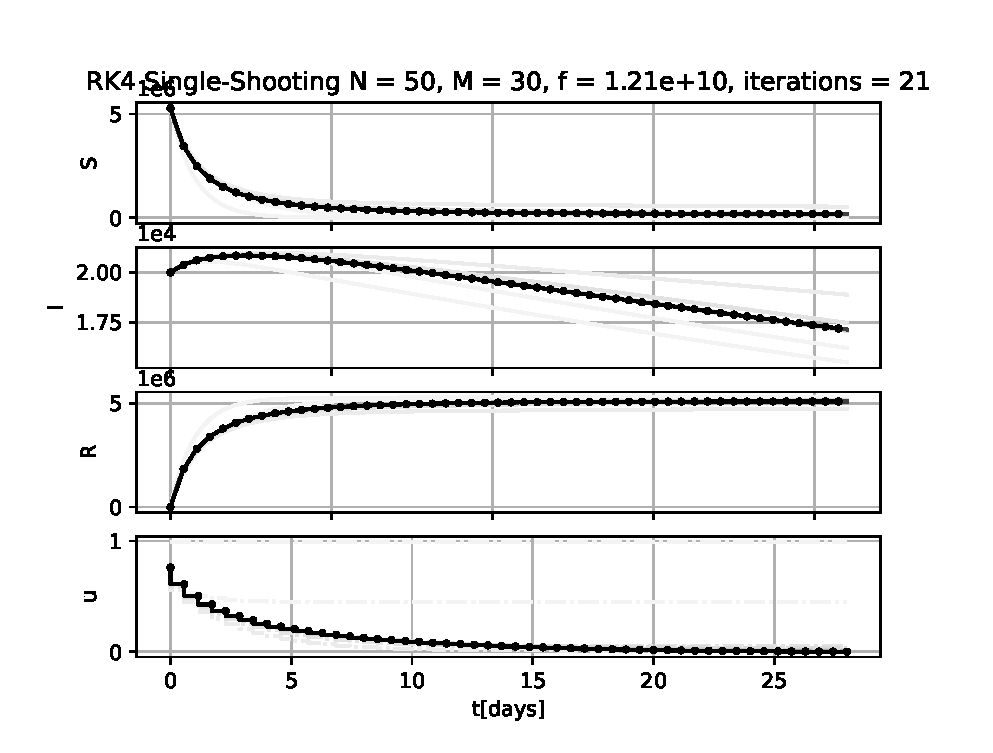
\includegraphics[width=.8\textwidth]{pythonProject/Figures/Single_Shooting_Trajectory_IPOPT.eps}
    \caption{Trajectories with single shooting using IPOPT}
    \label{fig:SH_Traj_IPOPT}
\end{figure}

\begin{figure}[H]
    \centering
    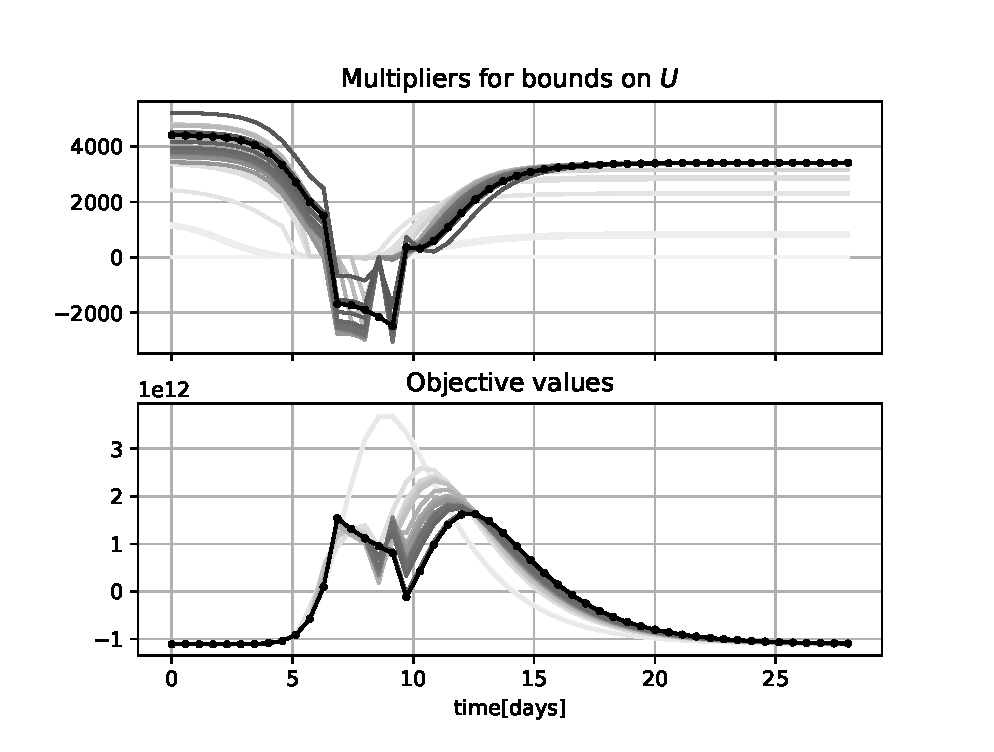
\includegraphics[width=.8\textwidth]{pythonProject/Figures/Single_Shooting_obj_con_IPOPT.eps}
    \caption{Bounds multipliers and objective values for single shooting using IPOPT (Social Distancing)}
    \label{fig:SH_con_obj_IPOPT}
\end{figure}
It is clear that the most cost-critical region $t\in [5, 10]$ is considered by the solver when it is searching for a solution. This region contains the highest objective values for the early iterations. The first iterations drastically reduce the objective values, 

\textbf{Note:} The IPOPT documentation does not explicitly explain the implementation of bounds, but the solver ensures that the optimization variables stays within them for all iterations. There is one multiplier for each pair of bounds, where the activeness of the bound is determined by the sign of the multiplier.

\subsection{Interfacing SQPOASES in CasADI}
\subsubsection{Implementation}
Passing 'sqpmethod' to $nlpsol(.)$ makes it possible to solve the same problem formulation as algorithm \ref{alg:SingleShooting_Integration_IPOPT}.

\subsubsection{Results}
Simulating with parameters defined in section \ref{ch:Problem_Parameters} yields trajectories shown in figure \ref{fig:} and multiplier and objective values shown in figure \ref{fig:SH_con_obj_IPOPT}.